\documentclass[aps, pra, signlecolumn, superscriptaddress, final, 11pt]{revtex4}
\pdfoutput=1


\usepackage[utf8]{inputenc}
\usepackage[T1]{fontenc}
\usepackage{amsmath}
\usepackage{amssymb}
\usepackage{float}
\usepackage{graphicx}
\usepackage{microtype}
\usepackage{tikz}



\newcommand{\abs}[1]{\left| #1 \right|}
\renewcommand{\theequation}{S.\arabic{equation}}
\renewcommand{\thefigure}{S.\arabic{figure}}


\begin{document}

\title{Cherenkov radiation and scattering of external dispersive waves by two-color solitons (Supplemental Material)}

\author{Ivan Oreshnikov}
\affiliation{Max Planck Institute for Intelligent Systems, Max-Planck-Ring 4, 72076 T\"ubingen, Germany}

\author{Oliver Melchert}
\affiliation{Cluster of Exellence PhoenixD, Welfengarten 1, 30167 Hannover, Germany}
\affiliation{Leibniz Universit\"at Hannover, Institute of Quantum Optics, Welfengarten 1, 30167 Hannover, Germany}
\affiliation{Hannover Centre for Optical Technologies, Nienburger Strasse 17, 30167 Hannover, Germany}

\author{Stephanie Willms}
\affiliation{Cluster of Exellence PhoenixD, Welfengarten 1, 30167 Hannover, Germany}
\affiliation{Leibniz Universit\"at Hannover, Institute of Quantum Optics, Welfengarten 1, 30167 Hannover, Germany}

\author{Surajit Bose}
\affiliation{Cluster of Exellence PhoenixD, Welfengarten 1, 30167 Hannover, Germany}
\affiliation{Leibniz Universit\"at Hannover, Institute of Photonics, Nienburger Strasse 17, 30167 Hannover, Germany}

\author{Ihar Babushkin}
\affiliation{Cluster of Exellence PhoenixD, Welfengarten 1, 30167 Hannover, Germany}
\affiliation{Leibniz Universit\"at Hannover, Institute of Quantum Optics, Welfengarten 1, 30167 Hannover, Germany}

\author{Ayhan Demircan}
\affiliation{Cluster of Exellence PhoenixD, Welfengarten 1, 30167 Hannover, Germany}
\affiliation{Leibniz Universit\"at Hannover, Institute of Quantum Optics, Welfengarten 1, 30167 Hannover, Germany}
\affiliation{Hannover Centre for Optical Technologies, Nienburger Strasse 17, 30167 Hannover, Germany}

\author{Uwe Morgner}
\affiliation{Cluster of Exellence PhoenixD, Welfengarten 1, 30167 Hannover, Germany}
\affiliation{Leibniz Universit\"at Hannover, Institute of Quantum Optics, Welfengarten 1, 30167 Hannover, Germany}
\affiliation{Hannover Centre for Optical Technologies, Nienburger Strasse 17, 30167 Hannover, Germany}

\author{Alexey Yulin}
\affiliation{Department of Physics, ITMO University, Kronverskiy pr. 49, 19701 St.~Petersburg, Russia}

\date{\today}

\maketitle

\section*{Dispersion profile model}

We model dispersion coefficient $\beta(\omega)$ with the following rational expression
\begin{equation}
  \label{eq:Beta}
  \beta(\omega) = \frac{1}{c} \frac{
    \sum_{n=0}^{3} {C_{n} \omega^{n+1}}
  }{
    \sum_{m=0}^{3} {D_{m} \omega^{m}}
    }
\end{equation}
where $c = 0.299792458~\mu
\text{m/fs}$ is the speed of light, and the coefficient sequences $C$ and $D$ are
defined by
\begin{eqnarray}
C &=& (9.654, -39.739 \,\mathrm{fs},  16.885 \,\mathrm{fs^2}, -2.746 \,\mathrm{fs^3}),\quad \text{and},\\
D &=& (1, -9.496 \,\mathrm{fs}, 4.221 \,\mathrm{fs^2}, -0.703 \,\mathrm{fs^3}).
\end{eqnarray}
%
In here and everywhere in the paper we assume fs as a unit of
time and $\mu$m as a unit of distance. Figure \ref{fig:Model} displays group
velocity $v_{g}(\omega) = 1 / \beta'(\omega)$ and second order dispersion
coefficient $\beta''(\omega)$ as functions of frequency. Frequencies
$\omega_{1}$ and $\omega_{2}$ correspond to the central frequencies of the
soliton's spectral components as chosen in the simulation corresponding to
Fig.\,1 of the paper.

\begin{figure}[ht]
  \centering
  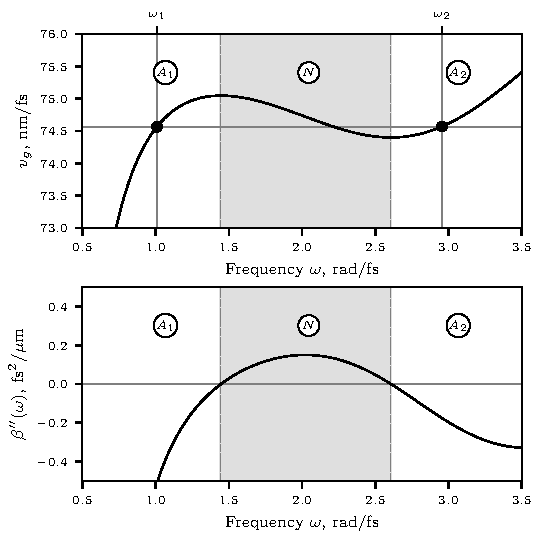
\includegraphics{{Figures/FigA}.pdf}
  \caption{
    (a) group velocity $v_{g}$ and (b) second order dispersion coefficient $\beta''(\omega)$ in the model fiber. Labels $A_{1,2}$ and $N$ mark the regions of anomalous and normal dispersion.
  }
  \label{fig:Model}
\end{figure}

\section*{Small internal oscillations of the soliton}

When analyzing the nonlinear scattering near an oscillatory mode we used an expression for the oscillation frequency. In this section we will derive this expression.

Let us return to Eq.~(3) (of the main text) for coupled solitons. We can re-normalize the equations by performing the following transformation
\begin{equation*}
  U_{n} \to \gamma_{n}^{1/2} e^{i \beta_{n} z} \cdot U_{n},
\end{equation*}
which will make the equations symmetric
\begin{equation*}
  i \partial_{z} U_{n}
    - \frac{1}{2} \beta''_{n} \partial_{t}^{2} U_{n}
    + \gamma_{n}^{2} \abs{U_{n}}^{2} U_{n}
    + 2 \gamma_{n} \gamma_{m} \abs{U_{m}}^{2} U_{n} = 0.
\end{equation*}
This in turn allows us to recognize the modified couple of equations as Euler-Lagrange equations for Lagrangian
\begin{equation*}
  \int \limits_{-\infty}^{+\infty}
    \mathcal{L}(U_{1}, \partial_{z} U_{1}, \partial_{t} U_{1}, \ldots)
    \, dt,
\end{equation*}
where Lagrangian density $\mathcal{L}$ is defined as a sum of three components $\mathcal{L} = \mathcal{L}_{1} + \mathcal{L}_{2} + \mathcal{L}_{\text{int}}$, with $\mathcal{L}_{n}$ being a single-soliton Lagrangian density
\begin{equation}
  \label{eq:SingleSolitonLagrangianDensity}
  \mathcal{L}_{n} =
  \frac{i}{2} \left(
    \partial_{z} U_{n} \cdot U_{n}^{*} -
    \partial_{z} U_{n}^{*} \cdot U_{n}
  \right)
  + \frac{1}{2} \beta''_{n} \, \partial_{t} U_{n} \partial_{t} U_{n}^{*}
  + \frac{1}{2} \gamma_{n}^{2} \, \abs{U_{n}}^{4},
\end{equation}
and $\mathcal{L}_{\text{int}}$ being the interaction term
\begin{equation}
  \label{eq:InteractionLagrangianDensity}
  \mathcal{L}_{\text{int}} =
    2 \gamma_{1} \gamma_{2}
    \abs{U_{1}}^{2} \abs{U_{2}}^{2}.
\end{equation}
Let us assume that the soliton components $U_{n}$ can be described by the following generic \textit{ansatz}
\begin{equation}
  \label{eq:SolitonAnsatz}
  U_{n}(z, t) = A_{n}(z) S\left(
    \frac{t - t_{n}(z)}{\sigma_{n}(z)}
  \right) \exp\left(
    - i \Omega_{n}(z) t + i \phi_{n}(z)
  \right).
\end{equation}
In here $A_{n}$ is the amplitude of the pulse, $t_{n}$ is the central position, $\sigma_{n}$ is the pulse width, $\Omega_{n}$ is the frequency detuning, $\phi_{n}$ is the phase, and $S(x)$ is function that defines the envelope shape. At the moment we will not specify the concrete form of $S(x)$, but will assume that it is an even function.

Before we continue let us stress one important thing: this ansatz cannot express all the possible internal oscillations of the soliton. One obvious example, as it was noted in the text, is the case of the pulse-width oscillation. In order to capture this dynamics, we need to add frequency chirp to the ansatz.

Substituting \eqref{eq:SolitonAnsatz} into \eqref{eq:SingleSolitonLagrangianDensity} and \eqref{eq:InteractionLagrangianDensity} and integrating over $t$ we arrive at the expressions for the averaged Lagrangians
\begin{gather}
  L_{n} =
    I_{1} \, t_{n} \sigma_{n} A_{n}^{2} \frac{d \Omega_{n}}{d z} +
    I_{1} \, \sigma_{n} A_{n}^{2} \frac{d \phi_{n}}{d z} +
    I_{2} \, \frac{\beta''_{n}}{2} \frac{A_{n}^{2}}{\sigma_{n}} \nonumber \\
    + I_{1} \, \frac{\beta''_{n}}{2} \sigma_{n} A_{n}^{2} \Omega_{n}^{2} +
    I_{3} \, \frac{\gamma_{n}^{2}}{2} \sigma_{n} A_{n}^{4} \\
  L_{\text{int}} =
    2 \, \gamma_{1} \gamma_{2} \, A_{1}^{2} A_{2}^{2} \,
    I_{\text{int}}(\sigma_{1}, \sigma_{2}, t_{1}, t_{2}),
\end{gather}
where the following integrals have been defined
\begin{align*}
  I_{1} =
    \int \limits_{-\infty}^{+\infty}
    S^{2}(x) \, dx &&
  I_{2} =
    \int \limits_{-\infty}^{+\infty}
    (S'(x))^{2} \, dx \\
  I_{3} =
    \int \limits_{-\infty}^{+\infty}
    S^{4}(x) \, dx &&
  I_{\text{int}} =
    \int \limits_{-\infty}^{+\infty}
    S^{2}\left(
      \frac{t - t_{1}}{\sigma_{1}}
    \right)
    S^{2}\left(
      \frac{t - t_{2}}{\sigma_{2}}
    \right) \, dt
\end{align*}
Due to the time invariance in the problem, $I_{\text{int}}$ depends only on the difference between $t_{1}$ and $t_{2}$
\begin{equation*}
  I_{\text{int}} = I_{\text{int}}(t_{1} - t_{2}, \sigma_{1}, \sigma_{2}),
\end{equation*}
and it is an even function of that difference.

The averaged Lagrangian $L = L_{1} + L_{2} + L_{\text{int}}$ is now a function defined in terms of soliton parameters \{\,$A_{n}$, $\sigma_{n}$, $t_{n}$, $\Omega_{n}$, $\phi_{n}$\,\} and only them. Therefore, the Euler-Lagrange equations for the new Lagrangian have to be defined in terms of variations over the soliton parameters
\begin{equation*}
  \frac{\delta L}{\delta P_{n}} =
    \frac{\partial{L}}{{\partial P_{n}}} -
    \frac{d}{dz} \frac{\partial L}{\partial \dot P_{n}} = 0,
\end{equation*}
where $P_{n}$ stands for either $A_{n}$, $\sigma_{n}$, $t_{n}$, $\Omega_{n}$ or $\phi_{n}$. The latter case --- variation with respect to the phase $\phi_{n}$ --- immediately yields the conservation of mass
\begin{equation}
  \label{eq:ConservationOfMass}
  N_{n} = \sigma_{n}(z) A_{n}^{2}(z) = \mathrm{const.}
\end{equation}

Variation with respect to the detuning $\Omega_{n}$ fixes the group velocity of individual solitons
\begin{equation}
  \label{eq:SolitonPosition}
  \frac{d t_{n}}{dz} = \beta''_{n} \Omega_{n}(z).
\end{equation}

Variation with respect to the soliton position $t_{n}$ gives us an equation for the frequency
\begin{equation}
  \label{eq:SolitonFrequency}
  \frac{d \Omega_{n}}{dz} =
    2 \cdot \frac{N_{m} \gamma_{1} \gamma_{2}}
           {I_{1} \sigma_{1}(z) \sigma_{2}(z)} \cdot
    \frac{\partial I_{\text{int}}}{\partial t_{n}}.
\end{equation}
The symmetry in the overlap integral $I_{\text{int}}$ with respect to the soliton positions $t_{1}$ and $t_{2}$ leads to conservation of momentum
\begin{equation}
  \label{eq:ConservationOfMomentum}
  N_{1} \Omega_{1}(z) + N_{2} \Omega_{2}(z) = \mathrm{const}.
\end{equation}

Finally, the difference between the variations with respect to $A_{n}$ and $\sigma_{n}$ gives us
\begin{equation}
  \label{eq:SolitonWidth}
  I_{2} \beta''_{n} +
  \frac{I_{3} \gamma_{n}}{2} N_{n} \sigma_{n}(z)
  + 2 N_{m} \gamma_{1} \gamma_{2} \frac{\sigma_{n}(z)}{\sigma_{m}(z)} \left(
    I_{\text{int}} + \sigma_{n} \frac{\partial I_{\text{int}}}{\sigma_{n}}
  \right) = 0.
\end{equation}
The very last equation --- omitted here --- is the evolution equation for the phase $\phi_{n}$. The right-hand's side of the equation is quite complicated, but since the phase does not occur anywhere in \eqref{eq:SolitonPosition}, \eqref{eq:SolitonFrequency} or \eqref{eq:SolitonWidth}, it is not important for the remaining analysis.

Let us switch from the the individual soliton positions to the mean position and the relative delay instead
\begin{align*}
  t_{0} = \frac{1}{2} \left(
    t_{1} + t_{2}
  \right) &&
  \Delta t = t_{1} - t_{2}
\end{align*}
Equation for the relative delay $\Delta t$
\begin{equation}
  \label{eq:RelativeDelay}
  \frac{d \Delta t}{dz} =
    \beta''_{1} \Omega_{1}(z) +
    \beta''_{2} \Omega_{2}(z)
\end{equation}
and equations \eqref{eq:SolitonFrequency} and \eqref{eq:SolitonWidth} form a closed system, with equations for $d \Delta t / dz$, $d \Omega_{n} / dz$ acting as equations of motion and equations \eqref{eq:SolitonWidth} fixing the widths $\sigma_{n}(z)$ as functions of $\Delta t$. By differentiating \eqref{eq:RelativeDelay} one more time and using \eqref{eq:SolitonFrequency} we get
\begin{equation*}
  \frac{d^{2} \Delta t}{dz^{2}} +
  2 \frac{
    \gamma_{1} \gamma_{2} \left(
      \beta''_{1} N_{1} + \beta''_{2} N_{2}
    \right)
  }{
    I_{1} \sigma_{1}(\Delta t) \sigma_{2}(\Delta t)
  } \frac{\partial}{\partial \Delta t}
  I_{\text{int}} (\Delta t, \sigma_{1}, \sigma_{2}) = 0
\end{equation*}
To transform this into a harmonic oscillator equation we need to linearize the second term around the equilibrium point $\Delta t = 0$. Since $I_{\text{int}}$ is an even function, the derivative $\partial I_{\text{int}} / \partial \Delta {t}$ is odd and it vanishes at $\Delta t = 0$. This means we can ignore $\Delta t$ dependency in $\sigma_{1}$ and $\sigma_{2}$ --- only the term proportional to $\partial^{2} I_{\text{int}} / \partial \Delta t^{2}$ will survive. Thus we finally arrive at
\begin{equation*}
  \frac{d^{2} \Delta t}{dz^{2}} +
  K_{0}^{2} \Delta t = 0,
\end{equation*}
where the resonance frequency $K_{0}$ is
\begin{equation}
  \label{eq:ResonanceFrequency}
  K_{0}^{2} = 2 \frac{
    \gamma_{1} \gamma_{2} \left(
      \beta''_{1} N_{1} + \beta''_{2} N_{2}
    \right)
  }{
    I_{1} \sigma_{1}(0) \sigma_{2}(0)
  } I_{\text{int}}''(0; \sigma_{1}(0), \sigma_{2}(0)).
\end{equation}

For a more concrete estimate let us finally consider a Gaussian envelope, i.e.~let us set $S(x) = \exp(-x^{2})$. Such a choice of the envelope shape fixes the integrals $I_{1} = \sqrt{\pi / 2}$ and
\begin{equation*}
  I_{\text{int}}(\Delta t, \sigma_{1}, \sigma_{2}) =
  \sqrt{ \frac{\pi}{2} }
  \frac{
    \sigma_{1} \sigma_{2}
  }{
    \sqrt{
      \left(
        \sigma_{1}^{2} + \sigma_{2}^{2}
      \right)
    }
  }
  \cdot \exp \left(
    \frac{
      -2 \Delta t^{2}
    }{
      \sigma_{1}^{2} + \sigma_{2}^{2}
    }
  \right),
\end{equation*}
which finally gives us the following expression for the resonance frequency
\begin{equation}
  \label{eq:ResonanceFrequencyGaussian}
  K_{0}^{2} =
    - \frac{
      8 \, \gamma(\omega_{1}) \gamma(\omega_{2})
    }{
      \left(
        \sigma_{1}^{2} + \sigma_{2}^{2}
      \right)^{3/2}
    } \cdot \left(
      \beta''(\omega_{1}) \sigma_{1} A_{1}^{2} +
      \beta''(\omega_{2}) \sigma_{2} A_{2}^{2}
    \right).
\end{equation}

\end{document}
